Now we have to define the set of instructions of the processor. Rather
than to list every single instruction it is easier to describe classes
of instructions with the same \emph{addressing mode}~\cite{mspmanual}
and partial order representation.

\textbf{ALU operation Rn to Rn}

An instruction from this class takes two operands stored in general
purpose registers $\{A,\ B\}$, performs an operation over them, and
writes the result back into one of them (so called \emph{register
direct addressing mode}). Examples: $\mathit{ADD\ A,\ B}$ -- addition
$A=A+B$; $\mathit{MOV\ B,\ A}$ -- assignment $B=A$. Figure~\ref{app-fig-Scenarios-of-8}(a)
shows the corresponding partial order of actions that have to be performed:
ALU works concurrently with PC increment (PCIU) and the next instruction
fetch (IFU) actions. As soon as both concurrent branches are completed,
the processor is ready to execute the next instruction. Note that
it is not important for the microcontroller which particular ALU operation
is being executed ($\mathit{ADD}$, $\mathit{MOV}$, or any other)
because the partial order of actions is not affected by this choice.
It is responsibility of ALU to detect which operation it has to perform
according to the current opcode. Therefore, it is sufficient to specify
only 8 behavioural scenarios of the microcontroller (as there are
8 classes of instructions).

\begin{figure}
\begin{centering}
\subfloat[ALU op. Rn to Rn]{

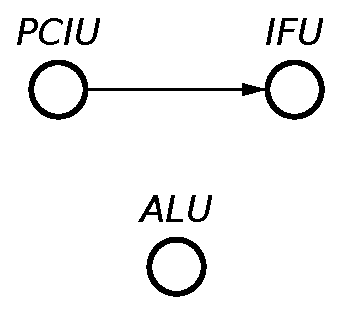
\includegraphics[scale=0.36]{fig/po_ALU_Rn_Rn}}\hfill{}\subfloat[ALU op. \#123 to Rn]{

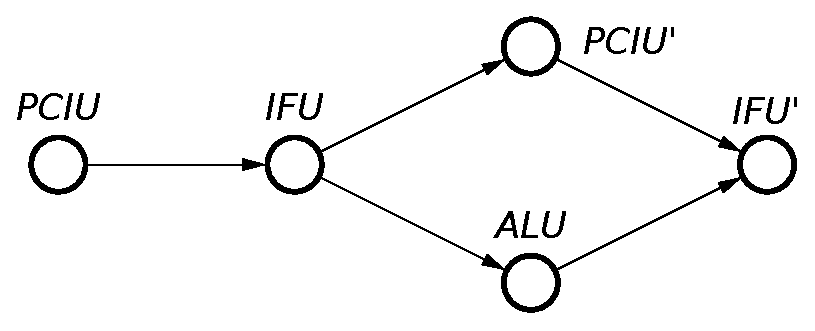
\includegraphics[scale=0.36]{fig/po_ALU_123_Rn}}\hfill{}\subfloat[ALU op. Rn to PC]{


\includegraphics[scale=0.36]{fig/po_ALU_Rn_PC}}\hfill{}\subfloat[ALU op. \#123 to PC]{

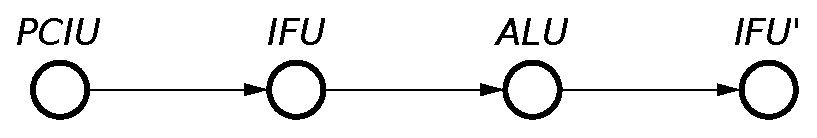
\includegraphics[scale=0.36]{fig/po_ALU_123_PC}}
\par\end{centering}

\begin{centering}
\subfloat[Memory access]{

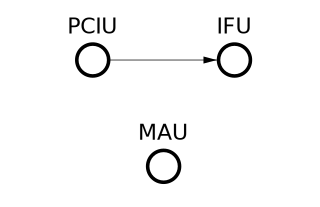
\includegraphics[scale=0.36]{fig/po_MAU}}\hfill{}\subfloat[Cond. ALU op. Rn to Rn]{

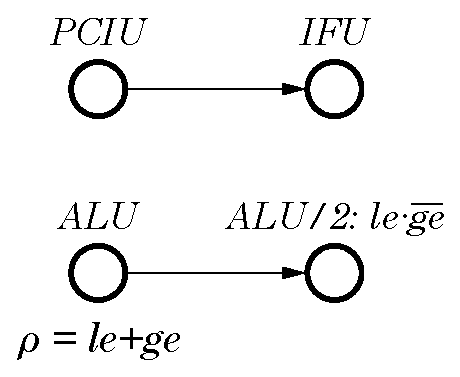
\includegraphics[scale=0.36]{fig/po_CALU_Rn_Rn}}\hfill{}\subfloat[Cond. ALU op. \#123 to Rn]{

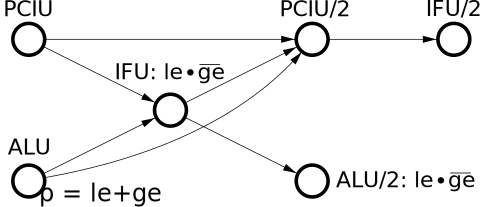
\includegraphics[scale=0.36]{fig/po_CALU_123_Rn}}\hfill{}\subfloat[Cond. ALU op. \#123 to PC]{

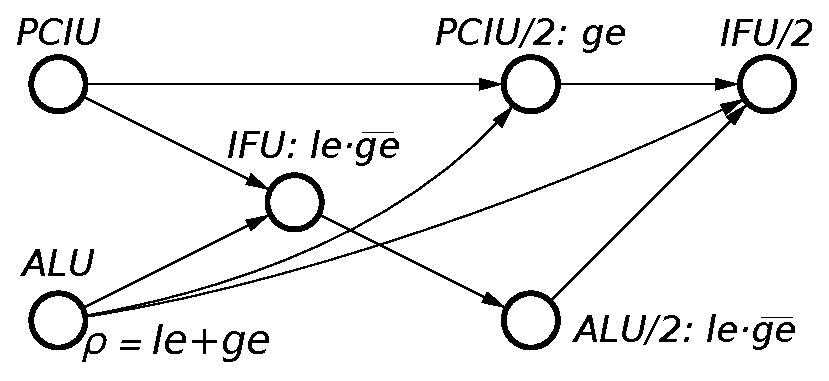
\includegraphics[scale=0.36]{fig/po_CALU_123_PC}}
\par\end{centering}

\caption{Conditional partial order specifications of 8 instruction classes\label{app-fig-Scenarios-of-8}}
\end{figure}


\textbf{ALU operation \#123 to Rn}

In this set of instructions one of the operands is register and another
is a constant which is given immediately after the instruction opcode
(e.g. $\mathit{SUB\ A,\ \#1}$ -- decrement $A$ by one), hence the
name: \emph{immediate addressing mode}. Figure~\ref{app-fig-Scenarios-of-8}(b)
shows the partial order of actions for such an instruction. At first,
the constant has to be fetched into IR (events PCIU and IFU). Then
ALU is executed concurrently with another increment of PC. Finally,
it is possible to fetch the next instruction into IR.

\textbf{ALU operation Rn to PC}

This class contains operations for unconditional branching, in which
PC register is modified. Branching can be absolute or relative: $\mathit{MOV\ PC,\ A}$
-- absolute branch to address stored in register $A$; $\mathit{ADD\ PC,\ B}$
-- relative branch to the address $B$ instructions ahead of the current
address. The partial order is very simple in this case: ALU is followed
with IFU -- see Figure~\ref{app-fig-Scenarios-of-8}(c).

\textbf{ALU operation \#123 to PC}

Instructions in this class are similar to those above with the exception
that the branch address is specified explicitly as a constant. The
actions should be scheduled in the following sequence: PCIU$\rightarrow$IFU
(to fetch the constant) followed by ALU and finally another IFU, as
shown in Figure~\ref{app-fig-Scenarios-of-8}(d).

\textbf{Memory access}

There are two instructions in this class: $\mathit{LOAD\ A}$ and
$\mathit{SAVE\ A}$. They load/save register $A$ from/to memory location
with address stored in register $B$. Figure~\ref{app-fig-Scenarios-of-8}(e)
shows that access to memory can be performed concurrently with the
next instruction fetch, exploiting the advantage of Harvard architecture.

\textbf{Conditional operations Rn to Rn, \#123 to Rn/PC}

These three classes of instructions are similar to their unconditional
versions above with the difference that they are performed only if
the following condition is true: $A<B$, i.e. register $A$ contains
a value which is less than that in register $B$. The first ALU action
compares registers $A$ and $B$, and changes ALU flags $\{le,\ ge\}$
according to the comparison result. These flags are thereafter checked
by the microcontroller in order to decide on the further scheduling
of actions. Consider, for example, conditional partial order in Figure~\ref{app-fig-Scenarios-of-8}(h).
It starts with concurrent increment of PC and comparison of registers
$A$ and $B$. If condition $A<B$ holds (i.e. $le\cdot\overline{ge}=1$)
then the process continues with the following sequence of actions:
IFU$\rightarrow$ALU/2$\rightarrow$IFU/2 (read the constant, perform
the branch, fetch the next instruction). Otherwise, the constant is
skipped (PCIU/2) and the next instruction is fetched (IFU/2). See~\cite{2009_mokhov_phd}
for details on dynamic CPOGs, which allow some of the operational
variables to be evaluated during execution of one of the scenarios
(in our case such dynamic variables are $\{le,\ ge\}$).

\begin{table}[h]
\centering

\begin{tabular}{|c||c|c|c|c|}
\hline 
\multirow{2}{*}{Instructions class} & 
\multirow{2}{*}{Trivial encoding} & 
\multicolumn{3}{c|}{ Optimal encoding} \tabularnewline
\cline{3-5}
& & $L=8$ & {$L=3$} & {$L=5$} \tabularnewline
\hline 
\hline 
{ ALU Rn to Rn} & { 000} & { 00000000} & { 000} & { 00000}\tabularnewline
\hline 
{ ALU \#123 to Rn} & { 001} & { 01001010} & { 110} & { 01001}\tabularnewline
\hline 
{ ALU Rn to PC} & { 010} & { 00010001} & { 101} & { 00010}\tabularnewline
\hline 
{ ALU \#123 to PC} & { 011} & { 01000010} & { 010} & { 01000}\tabularnewline
\hline 
{ Memory access} & { 100} & { 01000100} & { 100} & { 00100}\tabularnewline
\hline 
{ C/ALU Rn to Rn} & { 101} & { 00100000} & { 001} & { 10000}\tabularnewline
\hline 
{ C/ALU \#123 to Rn} & { 110} & { 10111010} & { 111} & { 11001}\tabularnewline
\hline 
{ C/ALU \#123 to PC} & { 111} & { 10110010} & { 011} & { 11000}\tabularnewline
\hline 
\end{tabular}

\caption{Synthesised instruction codes\label{tab:Synthesised-instruction-codes}}
\end{table}


